\documentclass[hidelinks,12pt,dvipsnames,border=2pt]{standalone}
%\usepackage[top=0.7in, bottom=0.8in, left=1in, right=1in]{geometry}
\usepackage{tikz}
\usepackage{hyperref}
\usetikzlibrary{arrows}
\usetikzlibrary{shapes}
\usepackage{enumitem}
\usepackage{bm}
\usepackage{mathdots}
\usepackage{amsmath}
\usepackage{tcolorbox}
\usetikzlibrary{shadings}
\usetikzlibrary{decorations.pathreplacing}
\usepackage{helvet}
\usepackage{url}
\usepackage{graphicx}
\usetikzlibrary{arrows.meta,positioning,fit,calc}
\renewcommand{\familydefault}{\sfdefault}


\usetikzlibrary{arrows,decorations.pathmorphing,backgrounds,fit,positioning,shapes.symbols,chains}

\begin{document}
	
% trim=left botm right top
\begin{tikzpicture}
\node at (0,0) {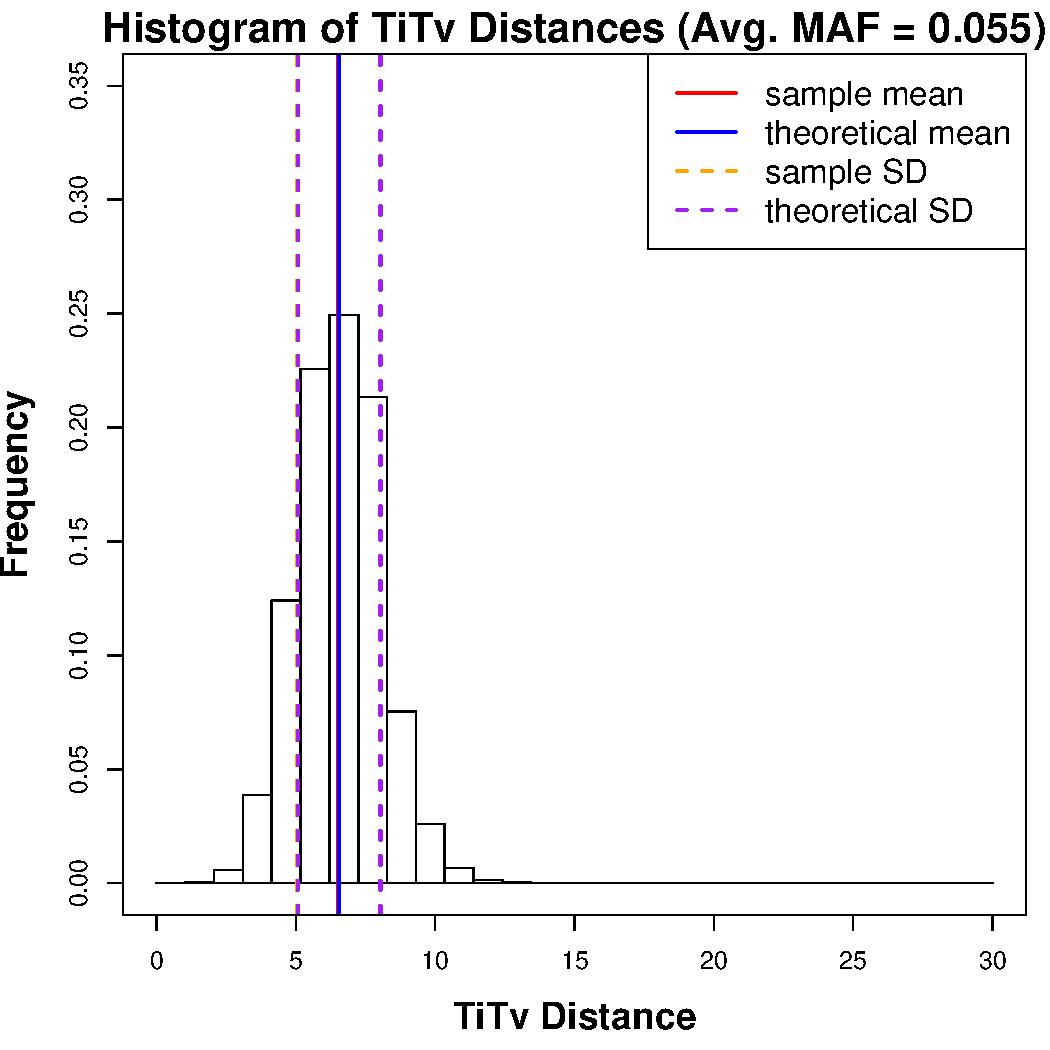
\includegraphics[width=\textwidth]{TiTv_distance_histogram_maf1.pdf}};

\node at (14,0) {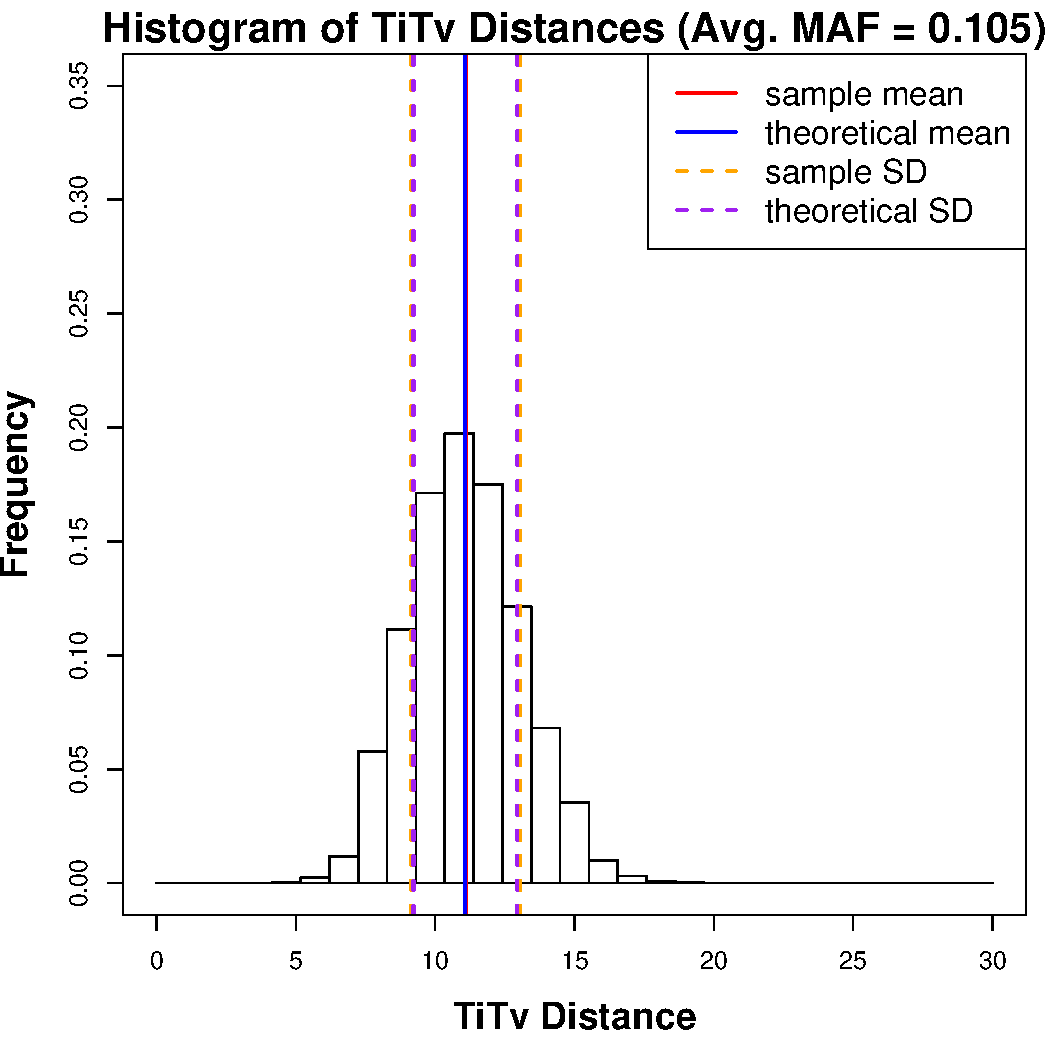
\includegraphics[width=\textwidth]{TiTv_distance_histogram_maf2.pdf}};

\node at (0,-14) {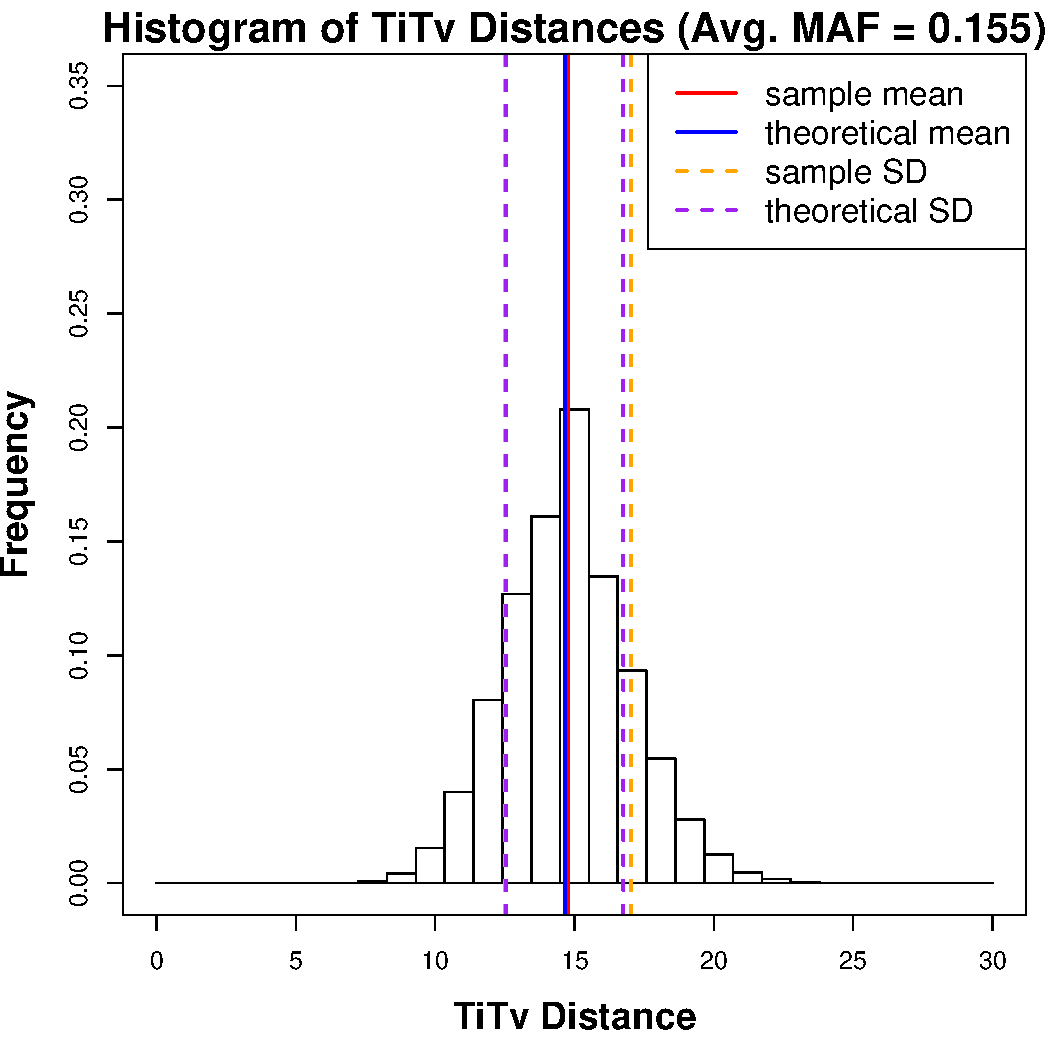
\includegraphics[width=\textwidth]{TiTv_distance_histogram_maf3.pdf}};

\node at (14,-14) {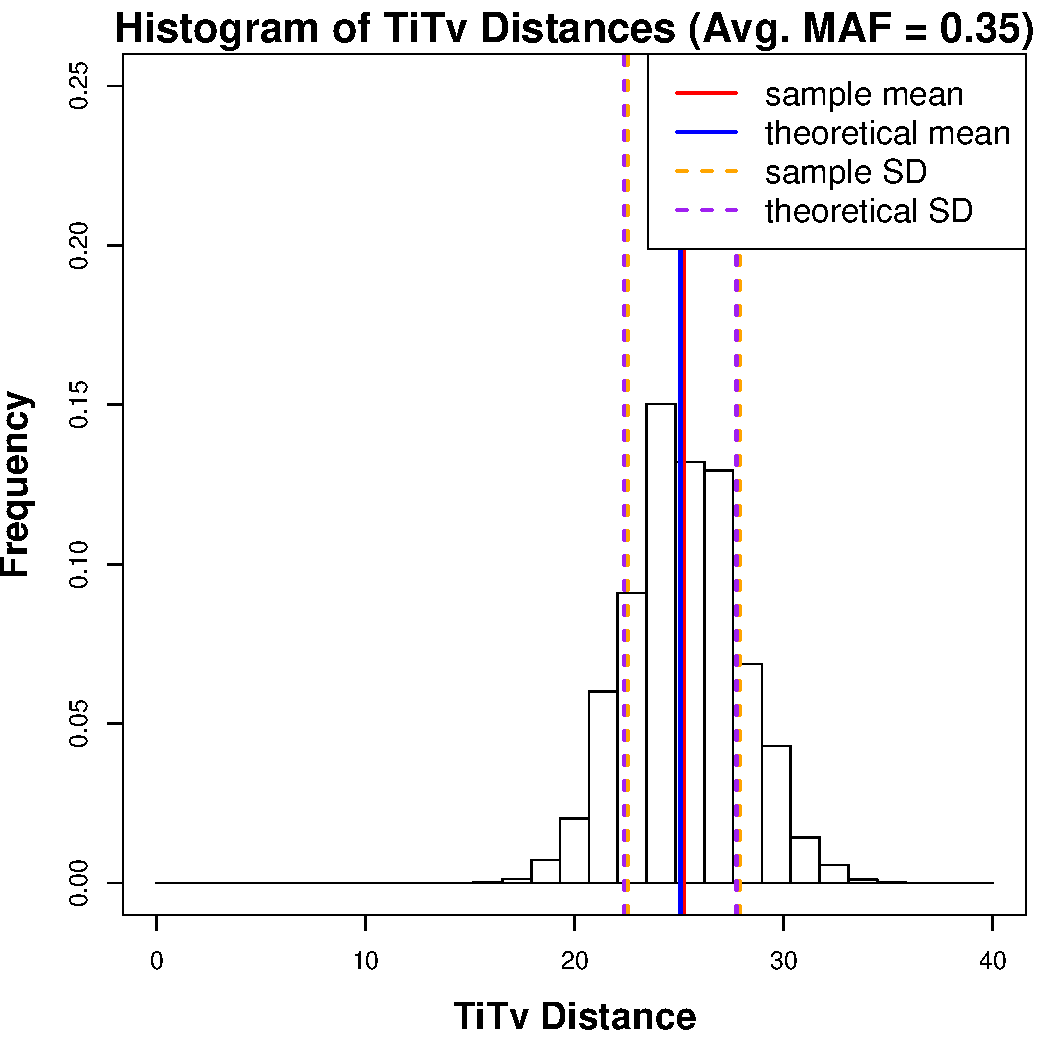
\includegraphics[width=\textwidth]{TiTv_distance_histogram_maf4.pdf}};
\end{tikzpicture}

\end{document}